\documentclass[border=6pt]{standalone}
\usepackage{tikz}
\usetikzlibrary{arrows.meta}
\begin{document}
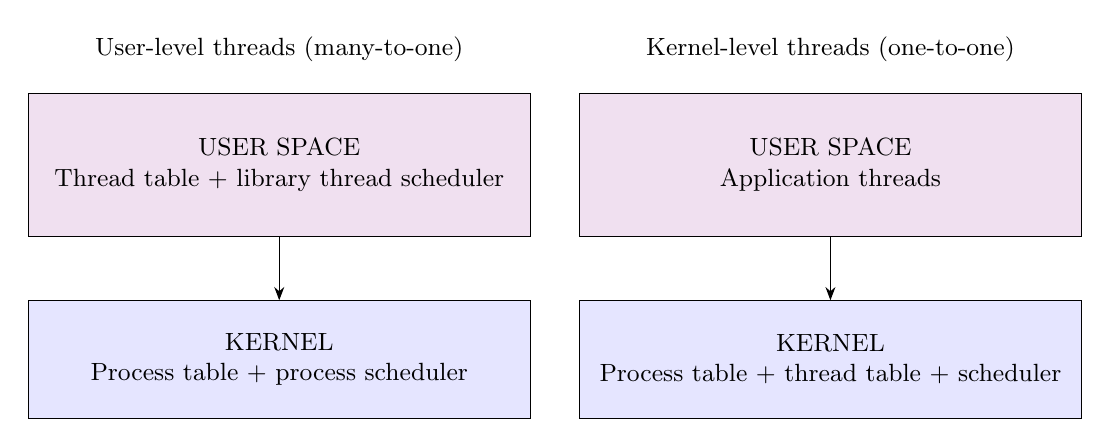
\begin{tikzpicture}[>=Stealth]
\node[align=center,font=\small] at (3.500,5.125) {User-level threads (many-to-one)};
\node[align=center,font=\small] at (10.500,5.125) {Kernel-level threads (one-to-one)};
\draw[fill=violet!12] (0.312,4.562) rectangle (6.688,2.750);
\node[align=center,font=\small] at (3.500,3.656) {USER SPACE\\Thread table + library thread scheduler};
\draw[fill=violet!12] (7.312,4.562) rectangle (13.688,2.750);
\node[align=center,font=\small] at (10.500,3.656) {USER SPACE\\Application threads};
\draw[fill=blue!10] (0.312,1.938) rectangle (6.688,0.438);
\node[align=center,font=\small] at (3.500,1.188) {KERNEL\\Process table + process scheduler};
\draw[fill=blue!10] (7.312,1.938) rectangle (13.688,0.438);
\node[align=center,font=\small] at (10.500,1.188) {KERNEL\\Process table + thread table + scheduler};
\draw[->] (3.500,2.750) -- (3.500,1.938);
\draw[->] (10.500,2.750) -- (10.500,1.938);
\end{tikzpicture}
\end{document}
